\documentclass{article}
\usepackage[margin=1in]{geometry}
\usepackage{problemset}
\showsolntrue

% Custom commands
\newcommand{\R}{\mathbb{R}}
\newcommand{\X}{\mathcal{X}}
\newcommand{\Y}{\mathcal{Y}}
\newcommand{\E}{\mathbb{E}}
\newcommand{\V}{\text{Var}}
\renewcommand{\P}{\mathbb{P}}

\begin{document}

\pstitle{%
    MATH 181A%
}{
    Homework 1%
}[due Saturday, January 10 at 11:59PM]

\begin{probset}
\begin{prob}[\textbf{3.6.6}]
    If
    \[f_Y(y) = \frac{2y}{k^2}, \quad 0 \leq y \leq k\]
    for what value of $k$ does $\V(Y) = 2$?

    \begin{soln}
        \[
            \V(Y) = \E[Y^2] - (\E[Y])^2
        \]
        \[
            \E[Y] = \int_0^k y \frac{2y}{k^2} dy = \frac{2}{k^2} \int_0^k y^2 dy = \frac{2}{k^2} \left[ \frac{y^3}{3} \right]_0^k = \frac{2k^3}{3k^2} = \frac{2k}{3}
        \]
        \[
            \E[Y^2] = \int_0^k y^2 \frac{2y}{k^2} dy = \frac{2}{k^2} \int_0^k y^3 dy = \frac{2}{k^2} \left[ \frac{y^4}{4} \right]_0^k = \frac{2k^4}{4k^2} = \frac{k^2}{2}
        \]
        \[
            \V(Y) = \frac{k^2}{2} - \left( \frac{2k}{3} \right)^2 = \frac{k^2}{2} - \frac{4k^2}{9} = \frac{9k^2 - 8k^2}{18} = \frac{k^2}{18}
        \]
        Setting this equal to 2, we get
        \[
            \frac{k^2}{18} = 2 \implies k^2 = 36 \implies k = 6
        \]
    \end{soln}
\end{prob}

\begin{prob}[\textbf{3.9.20}]
    Let $X$ be a binomial random variable based on $n$ trials and a success probability of $p_X$; let $Y$ be an independent binomial random variable based on $m$ trials and a success probability of $p_Y$. Find $\E[W]$ and $\V(W)$, where $W = 4X + 6Y$.

    \begin{soln}
        \[
            \E[W] = \E[4X + 6Y] = 4\E[X] + 6\E[Y] = 4np_X + 6mp_Y
        \]
        \[
            \V(W) = \V(4X + 6Y) = 4^2\V(X) + 6^2\V(Y) = 16np_X(1-p_X) + 36mp_Y(1-p_Y)
        \]
    \end{soln}
\end{prob}

\newpage

\begin{prob}[\textbf{3.10.6}]
    Let $Y_1, Y_2, \ldots, Y_n$ be a random sample from the exponential pdf $f_Y(y) = e^{-y}, y \geq 0$. What is the smallest $n$ for which $\P(Y_{\min} < 0.2) > 0.9$?

    \begin{soln}
        We have that
        \begin{align*}
            \P(Y_{\min} < 0.2) &= 1 - \P(Y_{\min} \geq 0.2) \\
            &= 1 - \P(Y_1 \geq 0.2, Y_2 \geq 0.2, \ldots, Y_n \geq 0.2) \\
            &= 1 - \prod_{i=1}^n \P(Y_i \geq 0.2) \\
            &= 1 - \prod_{i=1}^n \left( 1 - \int_0^{0.2} e^{-y} dy \right) \\
            &= 1 - \prod_{i=1}^n \left( 1 - (1 - e^{-0.2}) \right) \\
            &= 1 - e^{-0.2n} \geq 0.9 \\ 
            \implies 0.1 &\geq e^{-0.2n} \\
            \implies n &\geq \frac{\ln(0.1)}{-0.2} = 5\ln(10) \approx 11.5 \\ 
            \implies n &= 12
        \end{align*}
    \end{soln}
\end{prob}

\begin{prob}[\textbf{4.3.33}]
    The IQs of nine randomly selected people are recorded. Let $\bar Y$ denote their average. Assuming the distribution from which the $Y_i$'s were drawn is normal with a mean of 100 and a standard deviation of 16, what is the probability that $\bar Y$ will exceed 103? What is the probability that any arbitrary $Y_i$ will exceed 103? What is the probability that exactly three of the $Y_i$'s will exceed 103?

    \begin{soln}
        \[
            \P(\bar Y > 103) = \P\left( \frac{\bar Y - 100}{16/\sqrt{9}} > \frac{103 - 100}{16/\sqrt{9}} \right) = \P(Z > 0.5625) = 1 - \Phi(0.5625) \approx 0.2869
        \]
        \[
            \P(Y_i > 103) = 1 - \P\left( \frac{Y_i - 100}{16} < \frac{103 - 100}{16} \right) = 1 - \Phi(0.1875) \approx 1 - 0.5744 \approx 0.4256
        \]
        \[
            \P(\text{exactly 3 }Y_i > 103) = \binom{9}{3} \left( \P(Y_i > 103) \right)^3 \left( \P(Y_i \leq 103) \right)^6 = \binom{9}{3} (0.4256)^3 (0.5744)^6 \approx 0.2326
        \]
    \end{soln}
\end{prob}

\newpage

\begin{prob}[\textbf{4.3.34}]
    Let $Y_1, Y_2, \ldots, Y_n$ be a random sample from a normal distribution where the mean is 2 and the variance is 4. How large must $n$ be in order that
    $\P(1.9 \leq \bar Y \leq 2.1) \geq 0.99$

    \begin{soln}
        \begin{align*}
            \P(1.9 \leq \bar Y \leq 2.1) &= \P\left( \frac{1.9 - 2}{2/\sqrt{n}} \leq Z \leq \frac{2.1 - 2}{2/\sqrt{n}} \right) \\
            &= \P(-0.05\sqrt{n} \leq Z \leq 0.05\sqrt{n}) \\
            &= 2\Phi(0.05\sqrt{n}) - 1 \geq 0.99 \\
            \implies 0.995 &\leq \Phi(0.05\sqrt{n}) \\
            \implies 2.5758 &\leq 0.05\sqrt{n} \\
            \implies n &\geq (2.5758/0.05)^2 \approx 2653.898 \\
            \implies n &= 2654
        \end{align*}
    \end{soln}
\end{prob}

\begin{prob}
    Apply Chebyshev's inequality to prove the Weak Law of Large Numbers for the sample mean of i.i.d. random variables with a finite variance.

    \begin{soln}
        \begin{align*}  
            \P(|\bar X - \E[\bar X]| \geq \epsilon) &\leq \frac{\V(\bar X)}{\epsilon^2} \\
            \P\left( \left| \frac{X_1 + \cdots + X_n}{n} - \E[X_i] \right| \geq \epsilon \right) &\leq \frac{\V(\frac1n \sum_{i=1}^n X_i)}{\epsilon^2} = \frac{n\V(X_i)}{n^2\epsilon^2} = \frac{\V(X_i)}{n\epsilon^2} \\
            \implies \lim_{n \rightarrow \infty} \P\left( \left| \frac{X_1 + \cdots + X_n}{n} - \E[X_i] \right| \geq \epsilon \right) &\leq \lim_{n \rightarrow \infty} \frac{\V(X_i)}{n\epsilon^2} = 0
        \end{align*}
        Therefore, we have used Chebyshev's inequality to show that as $n$ grows, the Weak Law of Large Numbers holds, i.e. $\frac{X_1 + \cdots + X_n}{n} \rightarrow \E[X_i]$ in probability as probability of the difference between the sample mean and the expected value being greater than any $\epsilon > 0$ goes to 0.
    \end{soln}
\end{prob}

\newpage

\begin{prob}[\textbf{R Simulation}]
    Let $X_1, \ldots, X_n$ be i.i.d. random variables from a uniform distribution on $[0, 2]$. Generate and plot 10 paths of sample means from $n = 1$ to $n = 40$ in one figure for each case. Describe what you can observe from each plot and relate to the theory in this specific context to empirically check the Law of Large Numbers.

    \begin{subprobset}
    \begin{subprob}
        When n is large, $$\frac{X_1 + \cdots + X_n}{n} \text{ converges to } \E[X_i]$$

        \begin{soln}
            \begin{center}
                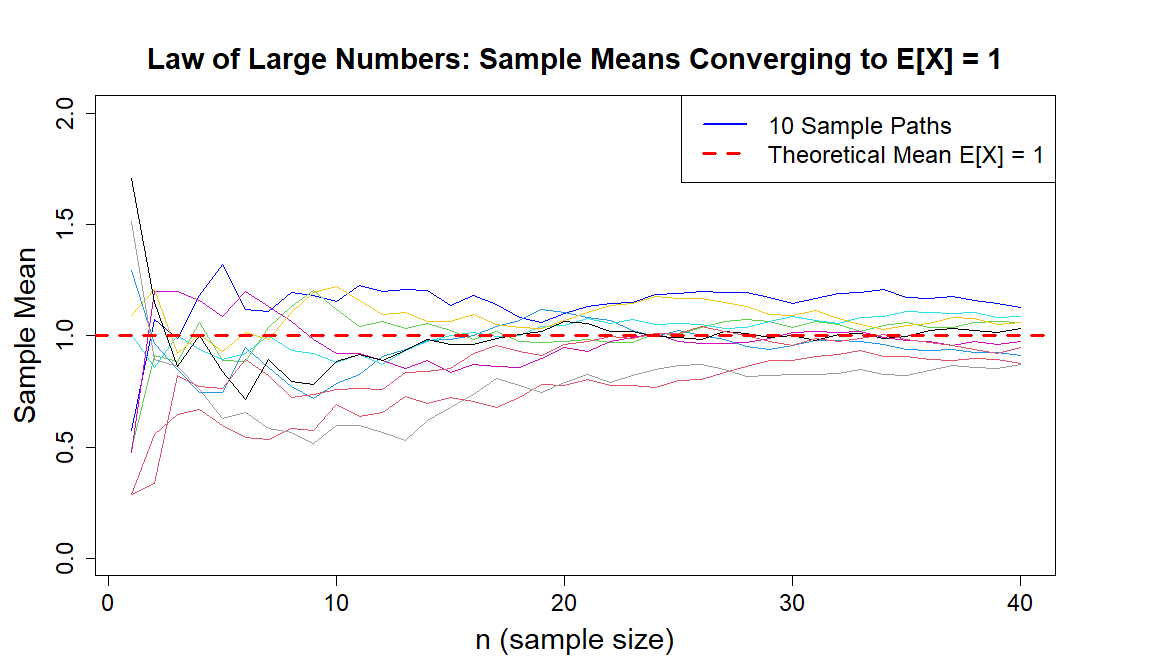
\includegraphics[width=0.6\textwidth]{Images/7.1.png}
            \end{center}
            As expected, the sample means converge to the theoretical mean of 1 as $n$ increases to 40 for all 10 paths. We can also observe that the variance of the sample means decreases as $n$ increases, starting very high and quickly descending to less than about 0.25 in 20 samples.
        \end{soln}
    \end{subprob}

    \begin{subprob}
        When n is large, $$\frac{X_1^2 + \cdots + X_n^2}{n} \text{ converges to } \E[X_i^2]$$

        \begin{soln}
            \begin{center}
                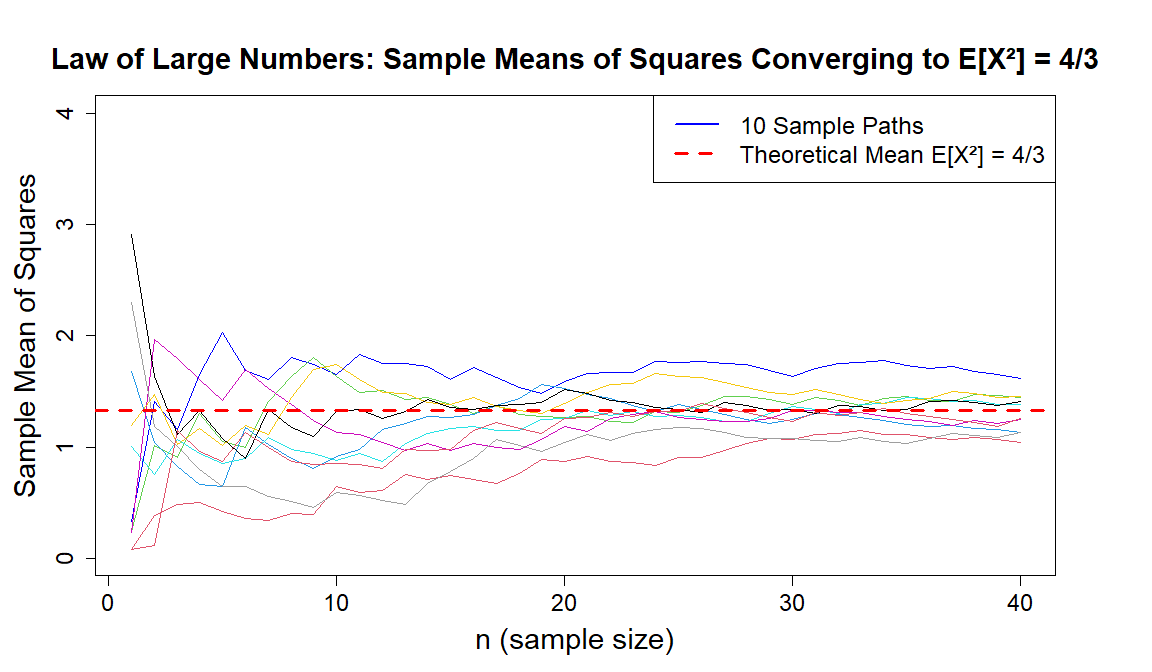
\includegraphics[width=0.6\textwidth]{Images/7.2.png}
            \end{center}
            Similarly, the sample means of squares converge to the theoretical mean of 4/3 as $n$ increases to 40 for all 10 paths. We can also observe that the variance of the sample means of squares decreases as $n$ increases. The main difference is that paths above the mean tend to be further than the ones below since the squares of the values are greater than the values themselves.
        \end{soln}
    \end{subprob}
    \end{subprobset}
\end{prob}
\end{probset}
\end{document}